\chapter{Features}
In this chapter, we will discuss the blocks and the states that we are going to support, design and implement.
% \section{Limitations}
% \begin{table}[H]
%     \caption{unsupported Blocks}
%     \centering
%   \begin{tabular}{ |m{26mm}|}
% \hline
% \rowcolor{Gray}
%  \multicolumn{1}{|c|}{\textbf{Unsupported Blocks}} 
% \\
% \hline


% 8/10b encoder \\ \hline 

% 128/130b encoder \\ \hline
% Serializer/ De-serializer \\ \hline
% Differential driver and receiver \\ \hline
% Elastic buffer logic \\ \hline 
% PLL (phase locked loop)
%  \\ \hline

% Lane de-skew delay circuit \\ \hline
% Block alignment and detect logic
%  \\ \hline
% Clock compensation \\ \hline
% \end{tabular}
% \end{table}
% \begin{table}[H]
%     \caption{unsupported states}
%     \centering
%   \begin{tabular}{ |m{26mm}|}
% \hline
% \rowcolor{Gray}
%  \multicolumn{1}{|c|}{\textbf{Unsupported States}} 
% \\
% \hline

% L1 \\ \hline 
%  L2 \\ \hline
% Hot Reset \\ \hline
% compliance  \\ \hline
% Loopback \\ \hline 
% Disable \\ \hline
% \end{tabular}

% \end{table}
\section{Supported Features}
\begin{table}[H]
    \caption{supported states}
    \centering
  \begin{tabular}{ |m{26mm}|}
\hline
\rowcolor{Gray}
\multicolumn{1}{|c|}{\textbf{
Supported States
} } \\
\hline

Detect \\ \hline 
Polling \\ \hline
Configuration\\ \hline
Recovery\\ \hline
L0\\ \hline 
L0s \\ \hline
\end{tabular}

\end{table}



\begin{table}[H]
    \caption{supported Blocks}
    \centering
  \begin{tabular}{ |m{26mm}|}
\hline
\rowcolor{Gray}
\multicolumn{1}{|c|}{\textbf{
Supported Blocks
} } 
\\
\hline


LPIF error handler \\ \hline 

LPIF control  \\ \hline
TxBuffer  \\ \hline
Ordered sets  \\ \hline
LTSSM  \\ \hline 
Byte Stripping / Unstripping 
 \\ \hline

Scrambler / De-scrambler  \\ \hline
PIPE register  
 \\ \hline
Arbiter/Mux \\ \hline
\end{tabular}
\end{table}


The LTSSM is composed of the following 11 states: Detect, Polling, Configuration, Recovery, L0, L0s, L1, L2, Hot Reset, Loopback, Disable. So here is a quick overview about the supported states:
\begin{enumerate}
    \item Detect \newline 
    It is the initial state of the physical layer, only used at Gen1 2.5 GT/s rate, or converted from the data link layer, or after reset, or from other states (Disable, Polling, Configuration, Recovery, etc.) Conversion. In short, the Detect state is the beginning of PCIe link training. In addition, Detect, as the name suggests, needs to implement detection work. Because in this state, the transmitting end TX needs to detect whether the receiving end RX exists and can work normally, if the detection is normal, it can enter other states. The Detect state mainly includes two sub-states: Detect.Quiet and Detect.Active.
    \item  Polling \newline 
    The purpose of this state is to "pair the cipher" and achieve barrier-free communication. After entering this state, the TS1 and TS2 OS sequences are sent between TX and RX to determine Bit Lock, Symbol Lock and solve the problem of Lane polarity reversal. The Polling state mainly includes three sub-states: Polling.Active, Polling.Configuration, Polling.Compliance.
    \item Configuration \newline 
    The content of this state is very simple. It is to determine the Link/Lane number by sending TS1 and TS2. Configuration contains 6 sub-states: Configuration.LinkWidth.Start, Configuration.LinkWidth.Accpet, Configuration.Lanenum.Wait, Configuration. Lanenum.Accpet, Configuration.Complete, Configuration.Idle

    \item Recovery \newline 
    When the PCIe link needs to be retrained, it enters the Recovery state. There are mainly the following situations:
\begin{itemize}
    \item When the PCIe link signal finds an error, the Bit Lock and Symbol Lock need to be adjusted

    \item  Exit from L0s state
    \item Speed Change. Because the first time you enter the L0 state, the rate is 2.5GT/s. When you need to adjust the rate to 5.0GT/s or 8.0GT/s, you need to enter the Recovery state for Speed Change. At this stage, Bit Lock, Symbol Lock, etc. Need to reacquire
    \item Need to readjust the Width of PCIe link
    \item Need to readjust the Width of PCIe link
    \item Only in Gen3 and Gen4, Equalization needs to be performed again.
\end{itemize}
    \item L0 \newline 
    This is the normal state (Normal and Full-Active State) of the link, and all TLP, DLLP and Ordered Sets can be sent and received normally. In this state, the rate can be 2.5GT/s or 5GT/s or higher (if the devices at both ends of the link support it and have undergone Re-Training).
    \item L0s \newline 
The ASPM (active-state power management) state is mainly used to reduce power consumption, and can enter this state when the bus is idle, and can quickly switch back to the L0 state from this state. When in the L0 state, when EIOS appears on the link, it means that it is about to enter the L0s state. When in the L0s state, when FTS appears on the link, the link will quickly complete bit lock and symbol lock, and enter the L0 state.
\end{enumerate}
\section{Supported Blocks}
\subsection{TxBuffer}
The ASPM (active-state power management) state is mainly used to reduce power consumption, and can enter this state when the bus is idle, and can quickly switch back to the L0 state from this state. When in the L0 state, when EIOS appears on the link, it means that it is about to enter the L0s state. When in the L0s state, when FTS appears on the link, the link will quickly complete bit lock and symbol lock, and enter the L0 state.
\subsection{Byte Stripping}
Bytes are striped across multiple lanes $\longrightarrow$ distribution of each byte to different lanes in turn to avoid different lanes with different data lengths.
%   \begin{figure}[H]
%   \centering
%   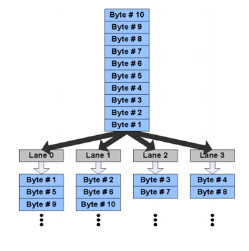
\includegraphics[width=80mm,height=80mm]{images/byte_str.png}
%   \caption{Byte Stripping}
  
%   \label{fig:pipe}
% \end{figure}
\subsection{Scrambler}
PCIe uses pseudo random data scrambling to spread off the RF energy in the frequency spectrum $\longrightarrow$ less electromagnetic interference (EMI). This is done by using a linear feedback shift registers on both the sender and receiver side. lfsr maintains an internal state machine which is the top flip-flops. An XOR operation is done between the state of the lfsr and the data $\longrightarrow$ resulting in a predictable and repeatable sequence of pseudo random data.
A parallel Scrambler performs 2 things: advance and apply. Advance means that the pattern changes, while apply means the XORing operation performed with this pattern.
\subsection{Ordered sets}
They are physical layer packets that only exists between Tx and Rx's physical layer.
\begin{itemize}
    \item TS1OS and TS2OS (Training Sequence 1 and 2)
    \item FTSOS (Fast Training Sequence)
    \item EIEOS (Electrical Idle Exit)
    \item EIOS (Electrical Idle)
    \item SOS (SKIP)
\end{itemize}
For more details about each block and how all the blocks interact together, see chapter \ref{4}.

% \begin{table}[H]
%     \caption{TX and Related signals}
%     \centering
%   \begin{tabular}{ |m{26mm}|m{10mm}|m{60mm}|  }
% \hline
% \rowcolor{Gray}
% \multicolumn{1}{|c|}{\textbf{Name} } 
% & \multicolumn{1}{|c|}{\textbf{Active Level}} 
% & \multicolumn{1}{|c|}{\textbf{Description}}\\
% \hline



% \end{tabular}
% \end{table}